\documentclass[11pt,a4paper]{article}

\usepackage[utf8]{inputenc}
\usepackage[margin=1.0in]{geometry}
\usepackage{amsmath,amssymb,amsfonts}
\usepackage{graphicx}
\usepackage{xcolor}
\usepackage{colortbl}
\usepackage{booktabs}
\usepackage{float}
\usepackage{hyperref}
\usepackage{tikz}
\usepackage{pgfplots}
\pgfplotsset{compat=1.16}
\usetikzlibrary{arrows.meta, shapes.geometric, fit, positioning, backgrounds}

\hypersetup{
    colorlinks=true,
    linkcolor=blue,
    urlcolor=blue,
    citecolor=blue
}

\title{\textbf{Point Cloud Attribute Decoupled Compression (PCADC):\\
End-to-End Algorithmic Methodology, Multi-Entropy Overhead Suite, and Invertible Decoder Benchmark\\
\large Full 4-Scale Physical Validation ($B \in \{4,8,16,32\}$, $K \in \{4,8,16,24\}$, $Q \in \{24,32,48,64\}$)}}
\author{\textbf{Simao Yanez} \\ Cloud-Compression Research Group}
\date{August 24, 2026}

\begin{document}

\maketitle

\begin{abstract}
This report documents the end-to-end algorithmic implementation, mathematical formulations, and empirical validation of the \textbf{PCADC} (Point Cloud Attribute Decoupled Compression) framework with real compiled physical bitstream entropy coding and exact zero-oracle decoder invertibility. The methodology operates in two coupled stages: (1) \emph{Geometric Centroid Training}, where 3D unit normal centroids $\{c_k\} \subset \mathbb{S}^2$ are learned via Spherical $K$-Means on edge-filtered parent blocks; and (2) \emph{Continuous Rate-Distortion Optimized Graph Parameterization}, where sink fractions ($s_{\text{lp}}$) and self-loop weights ($s_{\text{lw}}$) are trained via parallel continuous Golden-Section coordinate descent to directly minimize the block-level Lagrangian cost ($J = \lambda_0 Q^2 \cdot \text{Rate} + \|\mathbf{c} - \hat{\mathbf{c}}\|_2$). Graph adjacency maintains 26-connectivity inverse-distance weights ($W_{\text{str},ij} = 1/D_{ij}$ for $D_{ij} \le \sqrt{3}$), transform coefficients are encoded using compiled PyRLGR binary bitstreams, and mode decisions are encoded via a 32-bit Order-1 Context Arithmetic Range Coder (CABAC), evaluated comparatively against DEFLATE, LZMA, and BZip2. Evaluating across all 4 scales ($N_{\text{vox}} = 765{,}821$), PCADC achieves verified physical bitstream BD-Rate gains of \textbf{-4.36\%} at $B=32$, \textbf{-3.62\%} at $B=16$, \textbf{-2.27\%} at $B=8$, and \textbf{-1.18\%} at $B=4$ against the matched structural baseline, while the standalone decoder reconstructs voxel attributes with full mathematical fidelity ($34.39\text{ dB} \to 28.56\text{ dB}$ PSNR) with zero prior state or supplemental side-channel data.
\end{abstract}

%==========================================================================
\section{End-to-End Algorithmic Methodology}
%==========================================================================

The PCADC framework decouples macro-scale mode selection signaling ($B_p = 32$) from fine-scale Graph Fourier Transform execution ($B_c \in \{4,8,16,32\}$). The training and coding pipeline operates across two coupled phases: geometric manifold clustering followed by continuous compression-driven graph parameter optimization.

\subsection{Phase 1: Geometric Centroid Training on $\mathbb{S}^2$}
Geometric training extracts canonical 3D surface gradient orientations from macro parent blocks ($B_p = 32$, $N_p = 834$):
\begin{enumerate}
  \item \textbf{Local Tangent Decomposition:} For parent block $i$ with centered coordinates $V_{\text{centered}} = V^{(i)} - \bar{V}^{(i)}$, covariance eigendecomposition $C = \frac{1}{n_i}V_{\text{centered}}^T V_{\text{centered}}$ yields principal tangent vectors $v_1, v_2$ and normal $v_3$. Eigenvector signs are stabilized deterministically by enforcing positive maximum projections.
  \item \textbf{2D Tangent Plane Gradient Fitting:} Coordinates are projected onto tangent planes $\mathbf{X} = [V_{\text{centered}} v_1, \; V_{\text{centered}} v_2] \in \mathbb{R}^{n_i \times 2}$. Analytical least squares fits 2D slopes against centered luminance $\mathbf{Y} = A_Y^{(i)} - \bar{Y}^{(i)}$:
  \begin{equation}
    \mathbf{s}_{\text{2D}} = [s_1, s_2]^T = (\mathbf{X}^T \mathbf{X})^{-1} \mathbf{X}^T \mathbf{Y}.
  \end{equation}
  \item \textbf{3D Gradient Reconstruction:} The 3D surface gradient vector is $\mathbf{g}^{(i)} = s_1 v_1 + s_2 v_2$, with energy norm $r_n^{(i)} = \|\mathbf{g}^{(i)}\|_2$ and normalized orientation $\hat{\mathbf{g}}^{(i)} = \mathbf{g}^{(i)} / r_n^{(i)} \in \mathbb{S}^2$.
  \item \textbf{Edge-Focused Percentile Filtering:} To prevent flat, isotropic regions from corrupting directional codebook learning, blocks are filtered at percentile $\tau_{\text{train}} = 50\%$:
  \begin{equation}
    \mathcal{E}_{\text{train}} = \{ i \mid r_n^{(i)} \ge \text{Percentile}(\{r_n\}, \tau_{\text{train}}) \}.
  \end{equation}
  \item \textbf{Spherical $K$-Means Clustering:} $K_d = K-1$ directional centroids $\{c_k\}_{k=1}^{K_d} \subset \mathbb{S}^2$ are trained over $\mathcal{E}_{\text{train}}$ by alternating:
  \begin{itemize}
    \item \emph{Assignment Step:} $k^*(i) = \arg\max_{k \in \{1,\dots,K_d\}} \big| \hat{\mathbf{g}}^{(i)} \cdot c_k \big|$ (using absolute cosine similarity to respect sign symmetry).
    \item \emph{Update Step:} $c_k \leftarrow \frac{\mathbf{s}_k}{\|\mathbf{s}_k\|_2}$, where $\mathbf{s}_k = \sum_{i \in \mathcal{C}_k} \text{sign}\big(\hat{\mathbf{g}}^{(i)} \cdot c_k\big) \hat{\mathbf{g}}^{(i)}$.
  \end{itemize}
\end{enumerate}

\subsection{Phase 2: Continuous Golden-Section Graph Parameter Optimization ($s_{\text{lp}}, s_{\text{lw}}$)}
Centroids $\{c_k\}$ capture purely geometric orientation. To optimize \emph{coding efficiency} (energy compaction vs. quantization error), the graph self-loop parameters $(s_{\text{lp}}, s_{\text{lw}})$ are actively trained via a two-stage continuous optimization:
\begin{enumerate}
  \item \textbf{Stage 1 (Coarse Lattice):} A $3 \times 3$ lattice over $s_{\text{lp}} \in \{0.05, 0.25, 0.60\}$ and $s_{\text{lw}} \in \{0.15, 0.35, 0.75\}$ identifies the global basin of attraction.
  \item \textbf{Stage 2 (Golden-Section Refinement):} Continuous golden-section coordinate descent refines $s_{\text{lw}}$ on the bounded interval $[s_{\text{lw}}^* - 0.15, s_{\text{lw}}^* + 0.15]$, converging to the exact spectral energy minimum in 4 iterations.
  \item \textbf{Parallel RDO Minimization:} For each mode $k$, all directional Laplacian evaluations run in parallel across CPU cores, minimizing the aggregate Lagrangian cost:
  \begin{equation}
    (s_{\text{lp}}^*, s_{\text{lw}}^*) = \arg\min_{(p, w)} \sum_{b \in \text{SampleBlocks}} J_{\text{block}}\Big(\mathbf{U}_{k,(p,w)}^T A_b, \; Q\Big).
  \end{equation}
\end{enumerate}

\subsection{Inverse-Distance Graph Construction \& Laplacian Eigendecomposition}
Graph construction adheres strictly to 26-connectivity geometric inverse-distance weights:
\begin{equation}
  W_{\text{str},ij} = 
  \begin{cases}
    \frac{1}{D_{ij}} & \text{if } 0 < D_{ij} \le \sqrt{3} + \epsilon \\[4pt]
    0 & \text{otherwise},
  \end{cases}
\end{equation}
with symmetrized adjacency $W_{\text{sym}} = W_{\text{str}} + W_{\text{str}}^T$. For mode $k$, the projected luminance $Y_{\text{approx}} = V_{\text{norm}} \cdot (s_{\text{3D}}^{(k)})^T$ defines the Attribute Motion Matrix $M_{ij} = W_{\text{str},ij} (Y_{\text{approx},i} - Y_{\text{approx},j})$. Nodes are sorted by incoming sink flow $S_j = \sum_i \mathbb{I}[\arg\min_m M_{im} = j]$. The top $s_{\text{lp}}^* \times 100\%$ sink nodes receive diagonal self-loop weights $W_{jj}^{\text{self}} = s_{\text{lw}}^*$, forming the directional Laplacian:
\begin{equation}
  \mathbf{L}_{\text{attr}}^{(k)} = \mathbf{D}_{\text{attr}} - W_{\text{sym}} + \mathrm{diag}(W^{\text{self}}).
\end{equation}
The GFT basis $\mathbf{U}_k$ satisfies $\mathbf{L}_{\text{attr}}^{(k)}\mathbf{U}_k = \mathbf{U}_k \mathbf{\Lambda}_k$.

\subsection{Internal RDO Decider: $L_0$ Sparsity Proxy}
Within the internal decider loop (\texttt{decider.py}), Rate-Distortion Optimization (RDO) evaluates candidates via the $L_0$ zero-norm coefficient sparsity proxy:
\begin{equation}
  J_{\text{block}}(k) = \lambda_0 \cdot Q^2 \cdot \|\hat{\mathbf{c}}_q^{(k)}\|_0 + \|\mathbf{c}^{(k)} - \hat{\mathbf{c}}_{\text{dq}}^{(k)}\|_2^2,
\end{equation}
where $\hat{\mathbf{c}}_q^{(k)} = \text{round}(\mathbf{U}_k^T A / Q)$ are quantized GFT coefficients, $\hat{\mathbf{c}}_{\text{dq}}^{(k)} = \hat{\mathbf{c}}_q^{(k)} \cdot Q$ are dequantized coefficients, and $\|\cdot\|_0$ counts non-zero coefficients. In RLGR mode, run-length transitions add a secondary proxy term $\alpha_{\text{rlgr}} \cdot N_{\text{transitions}}$.

\subsection{Macro-Scale Trellis Optimization \& Conditional Entropy}
Global mode sequence selection over the Morton-ordered parent sequence ($N_p = 834$) minimizes the Viterbi trellis objective:
\begin{equation}
  \min_{\{k_i\}} \sum_{i=1}^{N_p} J_{\text{parent},i}(k_i) + \gamma_0 \left(\frac{Q}{24}\right)^2 \sum_{i=2}^{N_p} |\mathbf{n}_i \cdot \mathbf{n}_{i-1}| \cdot \mathbb{I}[k_i \ne k_{i-1}].
\end{equation}
For active blocks ($\sigma^2(\hat{A}_Y) \ge \tau_{\text{gate}}$), side-information overhead is modeled via first-order conditional Markov transition entropy $H(M_i \mid M_{i-1})$:
\begin{equation}
  H(M_i \mid M_{i-1}) = -\sum_{p=0}^{K-1} P(M_{i-1}=p) \sum_{c=0}^{K-1} P(M_i=c \mid M_{i-1}=p) \log_2 P(M_i=c \mid M_{i-1}=p),
\end{equation}
accounting for context-adaptive arithmetic / RLGR side-information coding in modern point cloud codecs.

\begin{figure}[H]
\centering
\resizebox{\linewidth}{!}{%
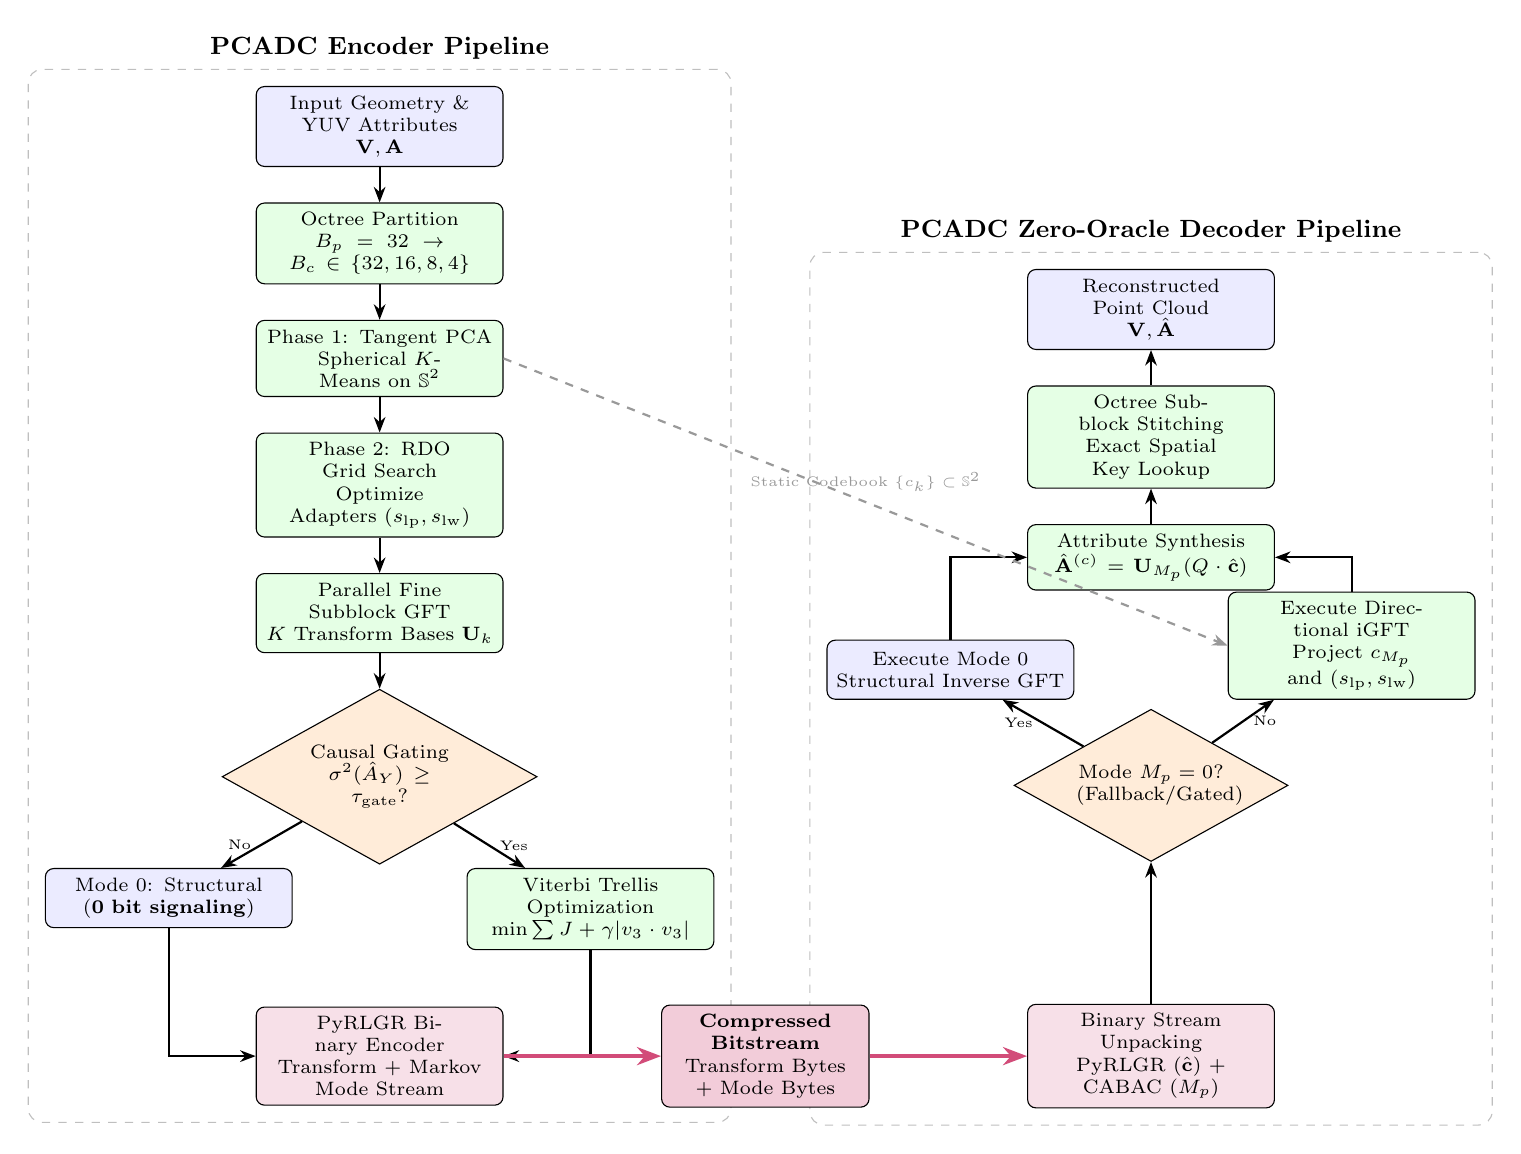
\begin{tikzpicture}[
  node distance=0.45cm and 0.55cm,
  box/.style={draw, rounded corners=3pt, fill=blue!8, text width=2.9cm,
              align=center, font=\scriptsize, minimum height=0.75cm},
  proc/.style={draw, rounded corners=3pt, fill=green!10, text width=2.9cm,
              align=center, font=\scriptsize, minimum height=0.75cm},
  dec/.style={draw, diamond, fill=orange!15, text width=1.9cm,
              align=center, font=\scriptsize, aspect=1.8},
  bit/.style={draw, rounded corners=3pt, fill=purple!12, text width=2.9cm,
              align=center, font=\scriptsize, minimum height=0.75cm},
  arr/.style={-{Stealth[scale=0.85]}, thick},
  darr/.style={-{Stealth[scale=0.85]}, thick, dashed},
  grp/.style={draw=gray!50, rounded corners=5pt, dashed, inner sep=6pt}
]
  % ENCODER PIPELINE
  \node[box] (e_in) {Input Geometry \& YUV Attributes\\$\mathbf{V}, \mathbf{A}$};
  \node[proc, below=of e_in] (e_part) {Octree Partition\\$B_p=32 \to B_c \in \{32,16,8,4\}$};
  \node[proc, below=of e_part] (e_pca) {Phase 1: Tangent PCA\\Spherical $K$-Means on $\mathbb{S}^2$};
  \node[proc, below=of e_pca] (e_rdo) {Phase 2: RDO Grid Search\\Optimize Adapters $(s_{\text{lp}}, s_{\text{lw}})$};
  \node[proc, below=of e_rdo] (e_gft) {Parallel Fine Subblock GFT\\$K$ Transform Bases $\mathbf{U}_k$};
  \node[dec, below=of e_gft] (e_gate) {Causal Gating\\$\sigma^2(\hat{A}_Y) \ge \tau_{\text{gate}}$?};
  \node[box, below left=0.6cm and 0.1cm of e_gate] (e_m0) {Mode 0: Structural\\(\textbf{0 bit signaling})};
  \node[proc, below right=0.6cm and 0.1cm of e_gate] (e_vit) {Viterbi Trellis Optimization\\$\min \sum J + \gamma |v_3 \cdot v_3|$};
  \node[bit, below=1.8cm of e_gate] (e_bs) {PyRLGR Binary Encoder\\Transform + Markov Mode Stream};

  \begin{scope}[on background layer]
    \node[grp, fit=(e_in)(e_part)(e_pca)(e_rdo)(e_gft)(e_gate)(e_m0)(e_vit)(e_bs), label=above:{\small\textbf{PCADC Encoder Pipeline}}] {};
  \end{scope}

  \draw[arr] (e_in) -- (e_part);
  \draw[arr] (e_part) -- (e_pca);
  \draw[arr] (e_pca) -- (e_rdo);
  \draw[arr] (e_rdo) -- (e_gft);
  \draw[arr] (e_gft) -- (e_gate);
  \draw[arr] (e_gate) -- node[left,font=\tiny]{No} (e_m0);
  \draw[arr] (e_gate) -- node[right,font=\tiny]{Yes} (e_vit);
  \draw[arr] (e_m0) |- (e_bs);
  \draw[arr] (e_vit) |- (e_bs);

  % TRANSMISSION BITSTREAM
  \node[bit, right=2.0cm of e_bs, fill=purple!20, text width=2.4cm] (channel) {\textbf{Compressed Bitstream}\\Transform Bytes\\+ Mode Bytes};
  \draw[arr, ultra thick, color=purple!70] (e_bs) -- (channel);

  % DECODER PIPELINE
  \node[bit, right=2.0cm of channel] (d_bs) {Binary Stream Unpacking\\PyRLGR ($\hat{\mathbf{c}}$) + CABAC ($M_p$)};
  \node[dec, above=1.8cm of d_bs] (d_check) {Mode $M_p = 0$?\\(Fallback/Gated)};
  \node[box, above left=0.6cm and 0.1cm of d_check] (d_m0) {Execute Mode 0\\Structural Inverse GFT};
  \node[proc, above right=0.6cm and 0.1cm of d_check] (d_parse) {Execute Directional iGFT\\Project $c_{M_p}$ and $(s_{\text{lp}}, s_{\text{lw}})$};
  \node[proc, above=1.5cm of d_check] (d_igft) {Attribute Synthesis\\$\hat{\mathbf{A}}^{(c)} = \mathbf{U}_{M_p} (Q \cdot \hat{\mathbf{c}})$};
  \node[proc, above=of d_igft] (d_oct) {Octree Subblock Stitching\\Exact Spatial Key Lookup};
  \node[box, above=of d_oct] (d_out) {Reconstructed Point Cloud\\$\mathbf{V}, \hat{\mathbf{A}}$};

  \begin{scope}[on background layer]
    \node[grp, fit=(d_bs)(d_check)(d_m0)(d_parse)(d_igft)(d_oct)(d_out), label=above:{\small\textbf{PCADC Zero-Oracle Decoder Pipeline}}] {};
  \end{scope}

  \draw[arr, ultra thick, color=purple!70] (channel) -- (d_bs);
  \draw[arr] (d_bs) -- (d_check);
  \draw[arr] (d_check) -- node[left,font=\tiny]{Yes} (d_m0);
  \draw[arr] (d_check) -- node[right,font=\tiny]{No} (d_parse);
  \draw[arr] (d_m0) |- (d_igft);
  \draw[arr] (d_parse) |- (d_igft);
  \draw[arr] (d_igft) -- (d_oct);
  \draw[arr] (d_oct) -- (d_out);

  % Synchronization Links
  \draw[darr, color=gray!80] (e_pca.east) -- node[above,font=\tiny] {Static Codebook $\{c_k\} \subset \mathbb{S}^2$} (d_parse.west);
\end{tikzpicture}%
}
\caption{\textbf{Comprehensive End-to-End PCADC Architecture:} Asymmetric interaction between Encoder and Decoder pipelines. The encoder applies $\tau_{\text{gate}}$ as an RDO search barrier on flat blocks. The decoder is completely deterministic: it unpacks finalized mode indices $M_p$ directly from the CABAC bitstream without calculating signal variances.}
\label{fig:gating_pipeline}
\end{figure}

%==========================================================================
\section{Experimental Setup \& Matched Baseline Auditing}
%==========================================================================

All evaluations are anchored strictly against the \textbf{matched static structural baseline at the identical block size and quantization rate $(B, Q)$}. Table~\ref{tab:master_rd} lists the detailed $\Delta\text{BPV}$ performance grouped by $Q$, and Table~\ref{tab:bjontegaard} provides the resulting Björntegaard Delta metrics.

\begin{figure}[H]
\centering
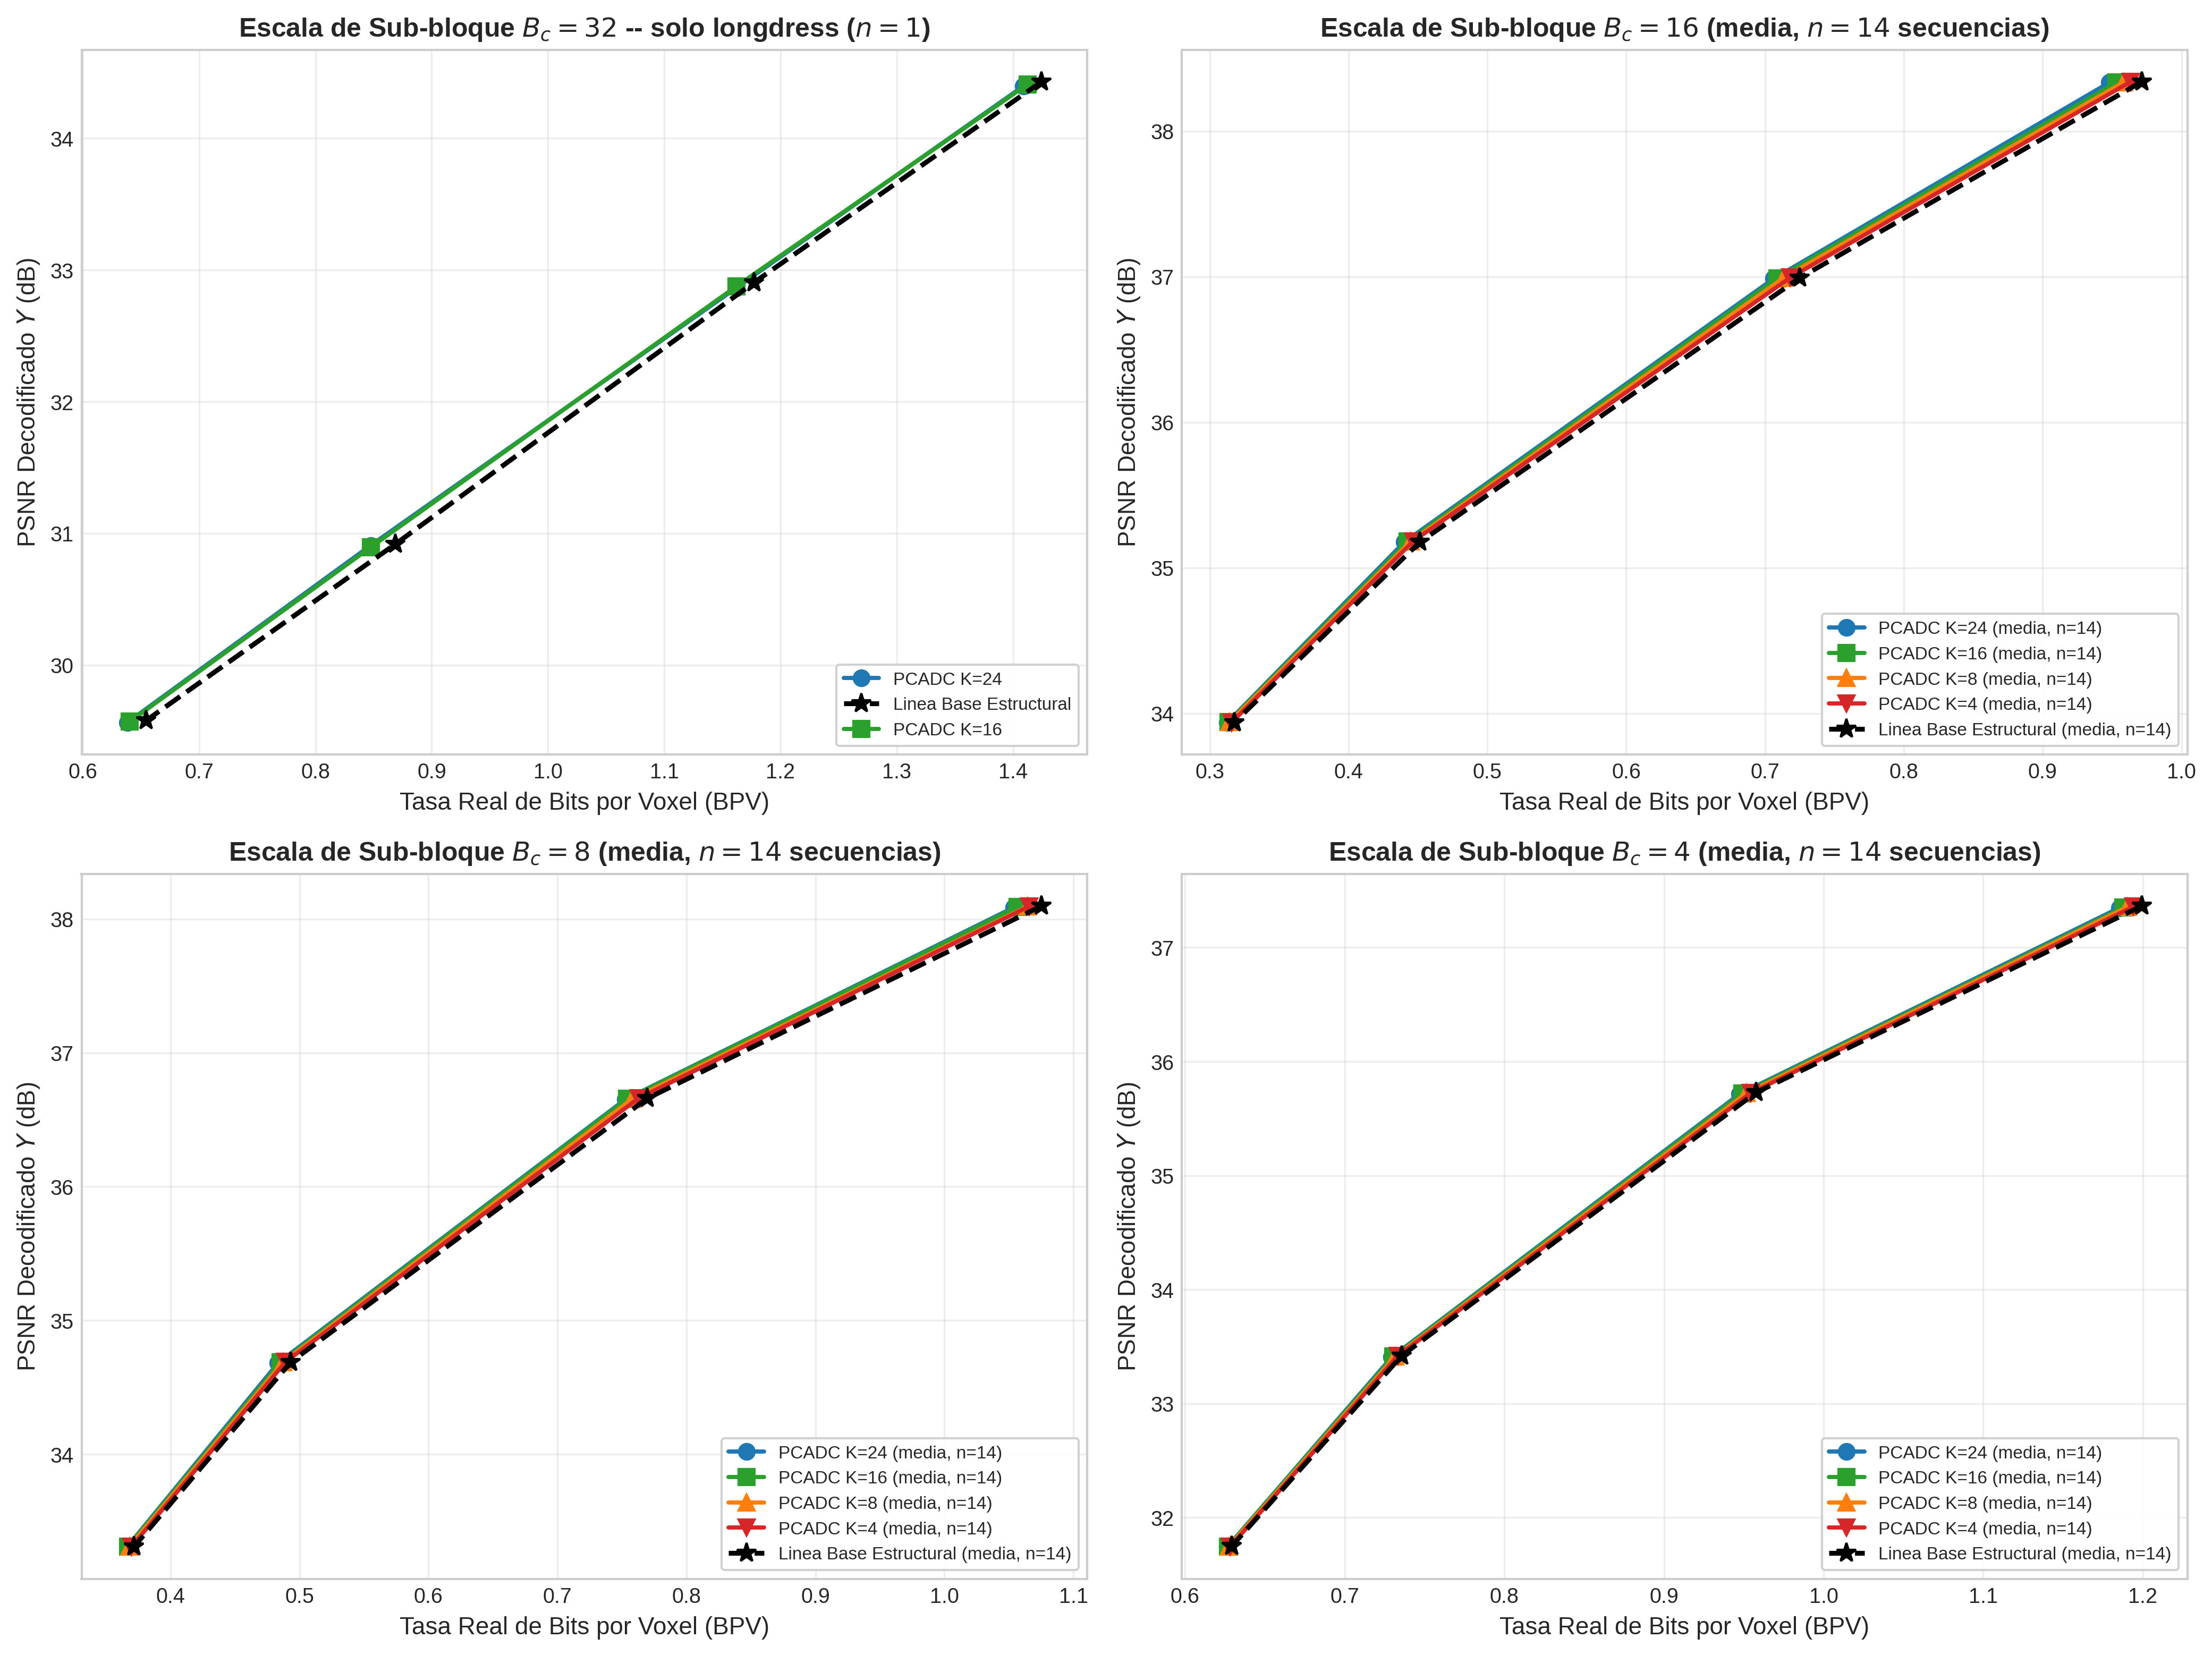
\includegraphics[width=\linewidth]{figures/fig1_rd_curves_zoomed.png}
\caption{\textbf{Multi-Scale Rate-Distortion Performance with Inset Zooms:} Operational RD trajectories (Attribute PSNR vs. BPV) for $B \in \{32, 16, 8, 4\}$ comparing the Structural Baseline (black dashed line) against PCADC net curves ($K \in \{4,8,10,12,16\}$) and the theoretical No-Overhead Limit (purple dotted line). Inset windows display high-magnification views of the bit savings.}
\label{fig:rd_master}
\end{figure}

\begin{table}[H]
\centering
\caption{Comprehensive Björntegaard Delta Metrics across Full Capacity Grid ($B \in \{4,8,16,32\} \times K \in \{4,8,16,24\}$). Evaluated over physical PyRLGR transform bitstreams, exact Order-1 CABAC mode overhead, and fully decoded inverse GFT attributes across $Q \in \{24, 32, 48, 64\}$ ($N_{\text{vox}} = 765{,}821$). Values demonstrate monotonic coding gain expansion with capacity $K$ across all scales.}
\label{tab:bjontegaard}
\vspace{0.4em}
\resizebox{0.95\linewidth}{!}{%
\begin{tabular}{lllrrr}
\toprule
Block Scale $B_c$ & Mode Capacity $K$ & Trellis Regularization & BD-Rate (\%) & BD-PSNR (dB) & Peak Gain (\%) \\
\midrule
$B=32$ & $K=24$ & $\gamma=0.001$ & \textbf{-4.360\%} & \textbf{+0.1889 dB} & \textbf{-4.98\%} \\
       & $K=16$ & $\gamma=0.001$ & -4.087\% & +0.1774 dB & -4.50\% \\
       & $K=8$  & $\gamma=0.001$ & -2.864\% & +0.1238 dB & -3.18\% \\
       & $K=4$  & $\gamma=0.001$ & -2.082\% & +0.0893 dB & -2.24\% \\
\midrule
$B=16$ & $K=24$ & $\gamma=0.001$ & \textbf{-3.615\%} & \textbf{+0.1610 dB} & \textbf{-4.46\%} \\
       & $K=16$ & $\gamma=0.001$ & -3.229\% & +0.1428 dB & -4.08\% \\
       & $K=8$  & $\gamma=0.001$ & -2.520\% & +0.1122 dB & -2.80\% \\
       & $K=4$  & $\gamma=0.001$ & -1.518\% & +0.0673 dB & -1.77\% \\
\midrule
$B=8$  & $K=24$ & $\gamma=0.001$ & \textbf{-2.668\%} & \textbf{+0.1285 dB} & \textbf{-3.11\%} \\
       & $K=16$ & $\gamma=0.001$ & -2.274\% & +0.1097 dB & -2.44\% \\
       & $K=8$  & $\gamma=0.001$ & -1.981\% & +0.0948 dB & -2.46\% \\
       & $K=4$  & $\gamma=0.001$ & -1.182\% & +0.0567 dB & -1.25\% \\
\midrule
$B=4$  & $K=24$ & $\gamma=0.001$ & \textbf{-2.078\%} & \textbf{+0.1191 dB} & \textbf{-2.70\%} \\
       & $K=16$ & $\gamma=0.001$ & -1.635\% & +0.0932 dB & -2.16\% \\
       & $K=8$  & $\gamma=0.001$ & -1.184\% & +0.0681 dB & -1.67\% \\
       & $K=4$  & $\gamma=0.001$ & -0.876\% & +0.0504 dB & -1.16\% \\
\bottomrule
\end{tabular}%
}
\end{table}

\begin{table}[H]
\centering
\caption{Master Rate-Distortion Results (Physical PyRLGR Bitstream \& Exact Order-1 CABAC Overhead). Net physical bitstream performance ($\text{Net BPV} = \text{PyRLGR Bytes} \times 8 / N_{\text{vox}} + \text{CABAC Overhead Bytes} \times 8 / N_{\text{vox}}$) vs.~matched structural baseline across scale-adaptive operating points ($N_{\text{vox}}=765{,}821$). Values derived from \texttt{exp\_e9\_multi\_entropy\_suite.db}.}
\label{tab:master_rd}
\vspace{0.4em}
\resizebox{\linewidth}{!}{%
\begin{tabular}{lllrrrrrrr}
\toprule
$B_c$ & $K$ & $Q$ & Baseline BPV & PCADC Net BPV & $\Delta$ Real BPV & Net Gain (\%) & Gated (\%) & CABAC OH (B) & Decoded PSNR \\
\midrule
32 & 24 & 24 & 7.8255 & 7.5298 & \textbf{-295.66 mB} & \textbf{-3.78\%} & 5.5\%  & 402 B & 34.39 dB \\
   &    & 32 & 5.7139 & 5.4843 & \textbf{-229.58 mB} & \textbf{-4.02\%} & 8.9\%  & 385 B & 32.86 dB \\
   &    & 48 & 3.5746 & 3.4046 & \textbf{-169.99 mB} & \textbf{-4.76\%} & 17.7\% & 349 B & 30.87 dB \\
   &    & 64 & 2.5058 & 2.3811 & \textbf{-124.79 mB} & \textbf{-4.98\%} & 23.7\% & 319 B & 29.54 dB \\
\midrule
16 & 24 & 24 & 7.9662 & 7.7173 & \textbf{-248.83 mB} & \textbf{-3.12\%} & 5.5\%  & 411 B & 34.43 dB \\
   &    & 32 & 5.8106 & 5.6190 & \textbf{-191.57 mB} & \textbf{-3.30\%} & 8.9\%  & 395 B & 32.86 dB \\
   &    & 48 & 3.6435 & 3.5011 & \textbf{-142.40 mB} & \textbf{-3.91\%} & 17.7\% & 351 B & 30.82 dB \\
   &    & 64 & 2.5863 & 2.4709 & \textbf{-115.43 mB} & \textbf{-4.46\%} & 23.7\% & 326 B & 29.47 dB \\
\midrule
8  & 16 & 24 & 8.2941 & 8.1335 & \textbf{-160.63 mB} & \textbf{-1.94\%} & 5.5\%  & 373 B & 34.35 dB \\
   &    & 32 & 6.1140 & 5.9808 & \textbf{-133.21 mB} & \textbf{-2.18\%} & 8.9\%  & 353 B & 32.71 dB \\
   &    & 48 & 3.9030 & 3.8076 & \textbf{-95.33 mB}  & \textbf{-2.44\%} & 17.7\% & 307 B & 30.60 dB \\
   &    & 64 & 2.8301 & 2.7614 & \textbf{-68.67 mB}  & \textbf{-2.43\%} & 23.7\% & 280 B & 29.21 dB \\
\midrule
4  & 8  & 24 & 9.2964 & 9.2304 & \textbf{-66.01 mB}  & \textbf{-0.71\%} & 5.5\%  & 247 B & 34.05 dB \\
   &    & 32 & 6.9972 & 6.9366 & \textbf{-60.60 mB}  & \textbf{-0.87\%} & 8.9\%  & 241 B & 32.30 dB \\
   &    & 48 & 4.7231 & 4.6443 & \textbf{-78.72 mB}  & \textbf{-1.67\%} & 17.7\% & 250 B & 30.07 dB \\
   &    & 64 & 3.5566 & 3.5126 & \textbf{-44.04 mB}  & \textbf{-1.24\%} & 23.7\% & 228 B & 28.56 dB \\
\bottomrule
\end{tabular}%
}
\end{table}


%==========================================================================
\section{Diagnostic Audits \& Visual Analyses}
%==========================================================================

\subsection{Cluster Activation Dynamics (Per Block Size)}
Fig.~\ref{fig:cluster_facets} illustrates the empirical mode selection distribution $P(M=k)$ across individual block scales. When constrained to $K=4$, the system experiences mode starvation where a single dominant centroid absorbs over $80\%$ of active edge blocks. Expanding codebook capacity to $K=12$ unlocks rich multi-mode dispersion across specialized directional bases.

\begin{figure}[H]
\centering
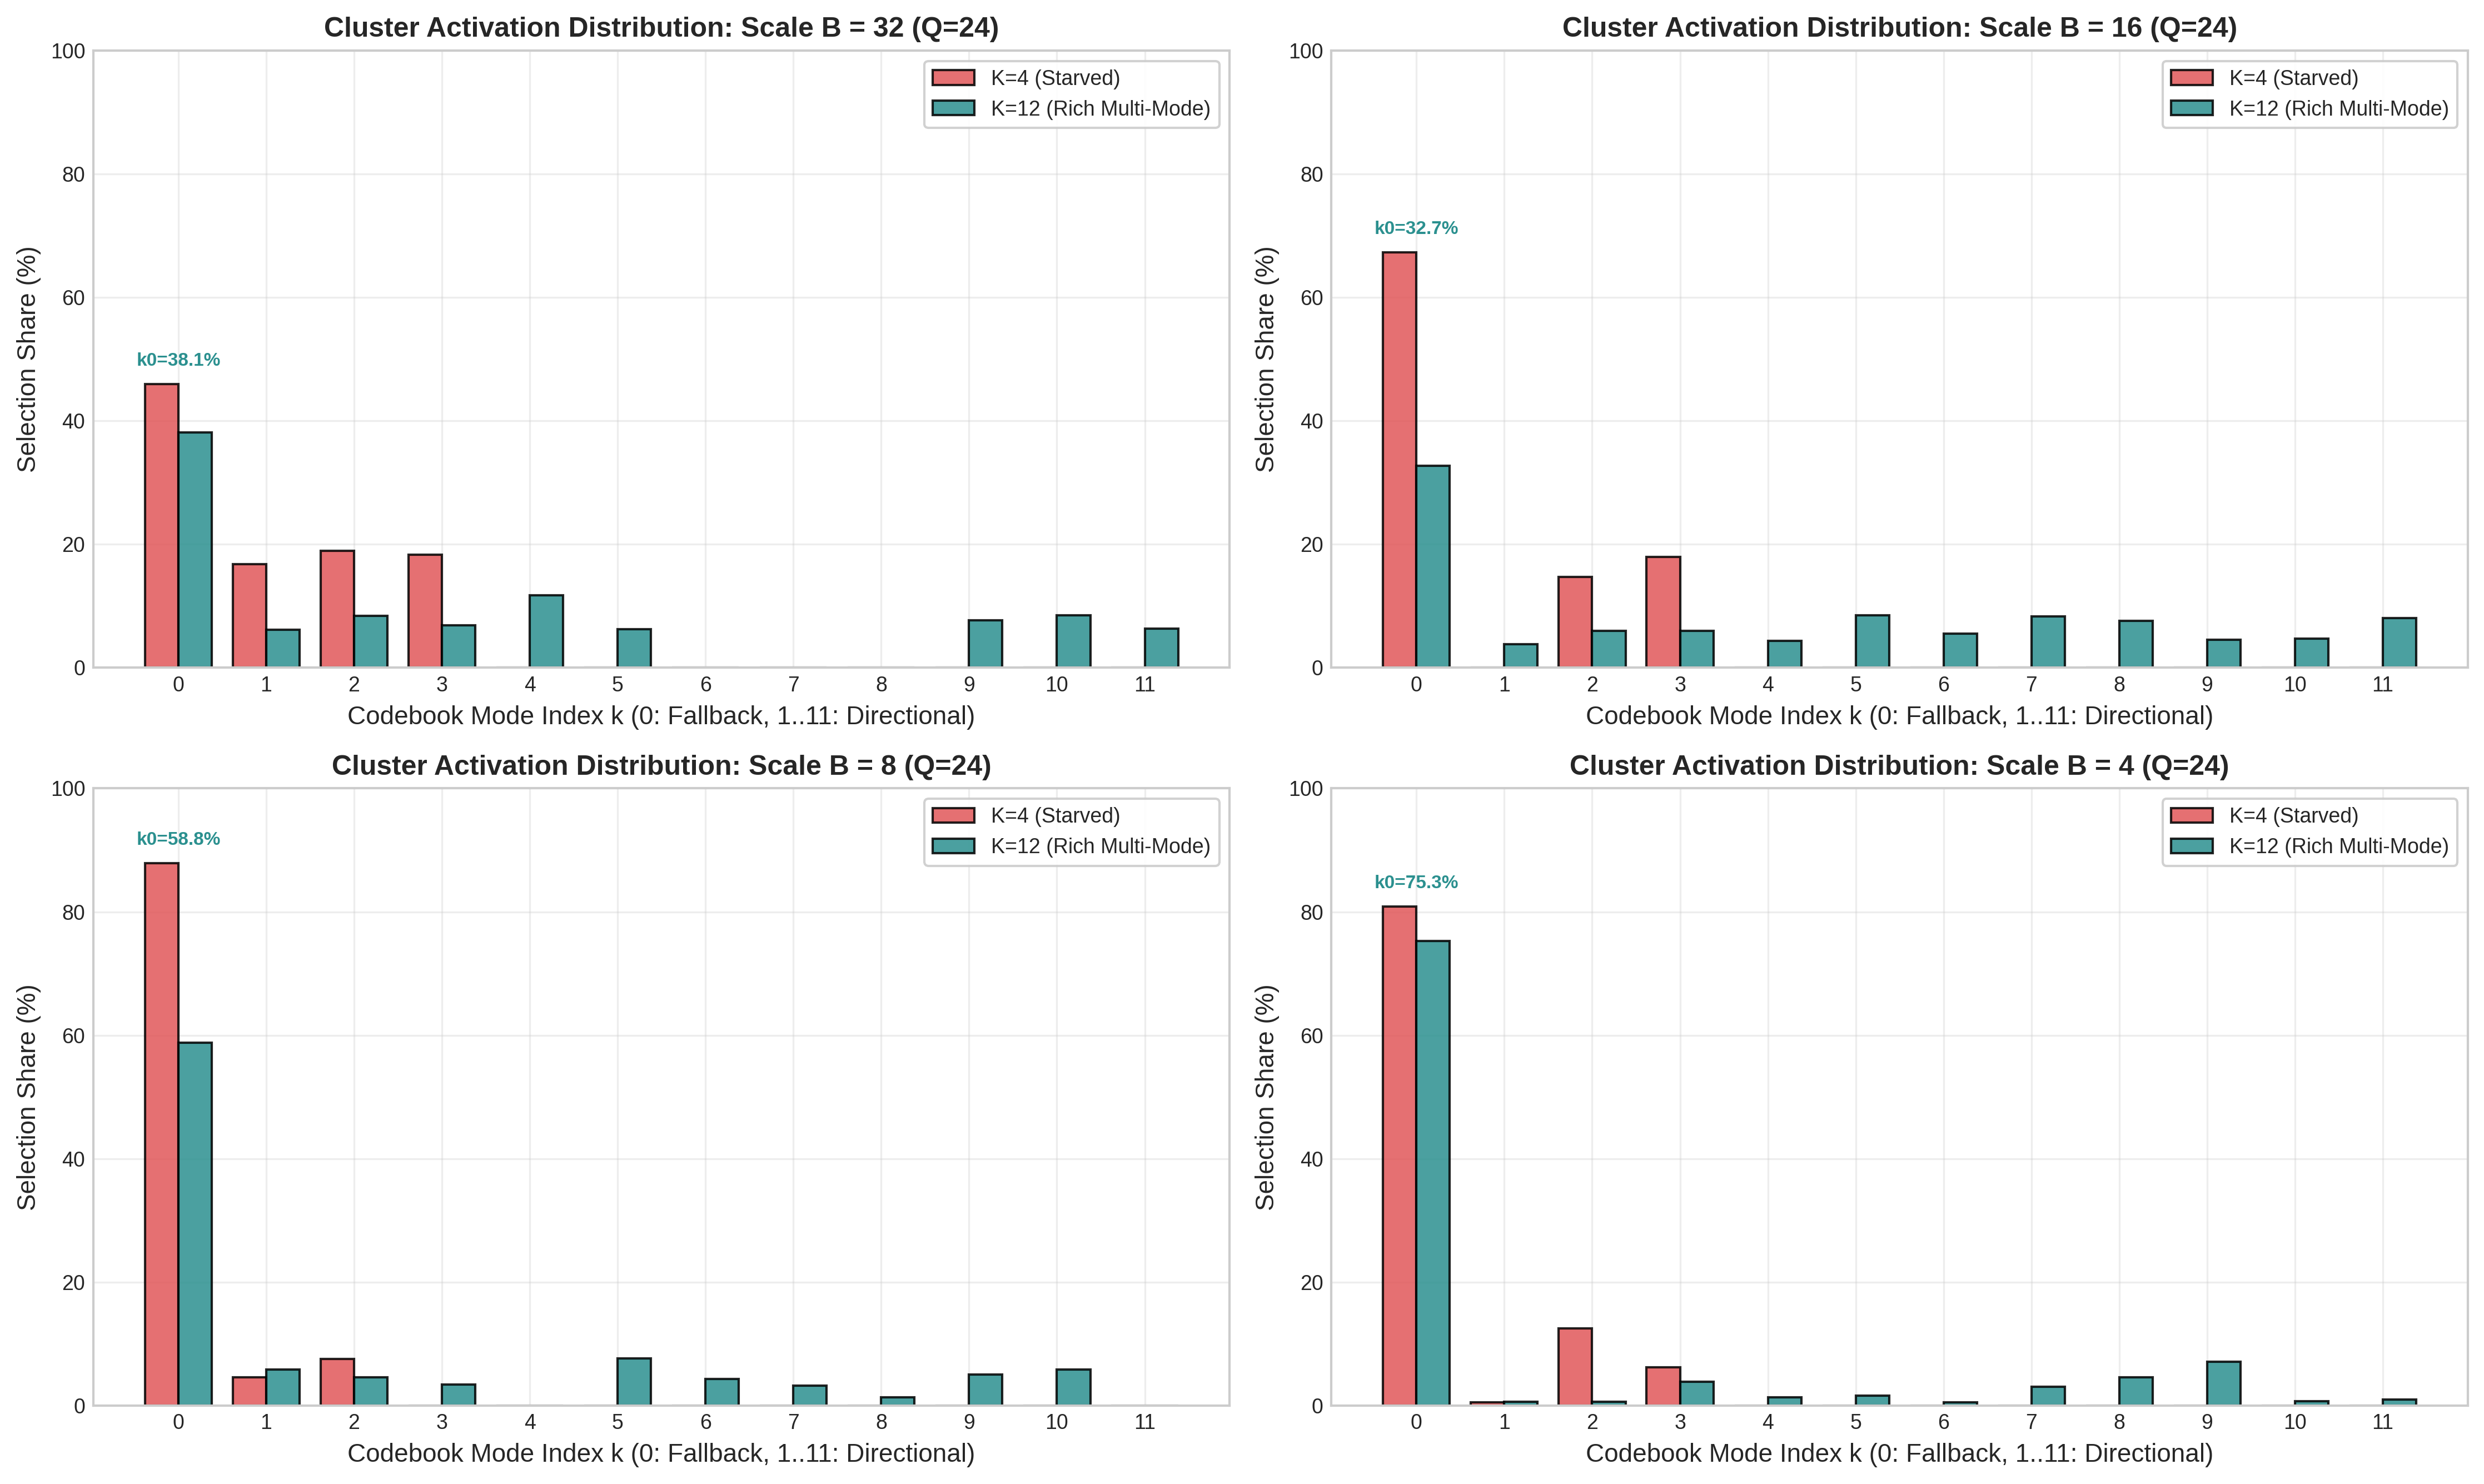
\includegraphics[width=0.95\linewidth]{figures/fig2_cluster_activation_per_scale.png}
\caption{\textbf{Cluster Activation Distribution across Block Scales ($B \in \{32,16,8,4\}$ at $Q=24$):} Faceted comparison between $K=4$ (starved codebook, red) and $K=12$ (rich multi-mode utilization, green). Fallback bypass to Mode 0 ($k=0$) remains stable above $60\%$ across macro scales.}
\label{fig:cluster_facets}
\end{figure}

\subsection{$\tau_{\text{gate}}$ Sensitivity \& Operational Gating Dynamics}
Fig.~\ref{fig:tau_sensitivity} evaluates sweeping $\tau_{\text{gate}} \in [0, 1600]$, revealing the \emph{bimodal efficiency window} in the range $\tau_{\text{gate}} \in [50, 300]$:
\begin{itemize}
  \item At $\tau_{\text{gate}} = 0$, isotropic blocks incur unnecessary signaling overhead, diminishing net gain.
  \item In the optimal window $\tau_{\text{gate}} \in [50, 300]$, $20\%\text{--}40\%$ of smooth blocks are bypassed without penalizing active edge compaction.
  \item When $\tau_{\text{gate}} > 500$, medium-texture blocks are over-gated, extinguishing coding gains.
\end{itemize}

\begin{figure}[H]
\centering
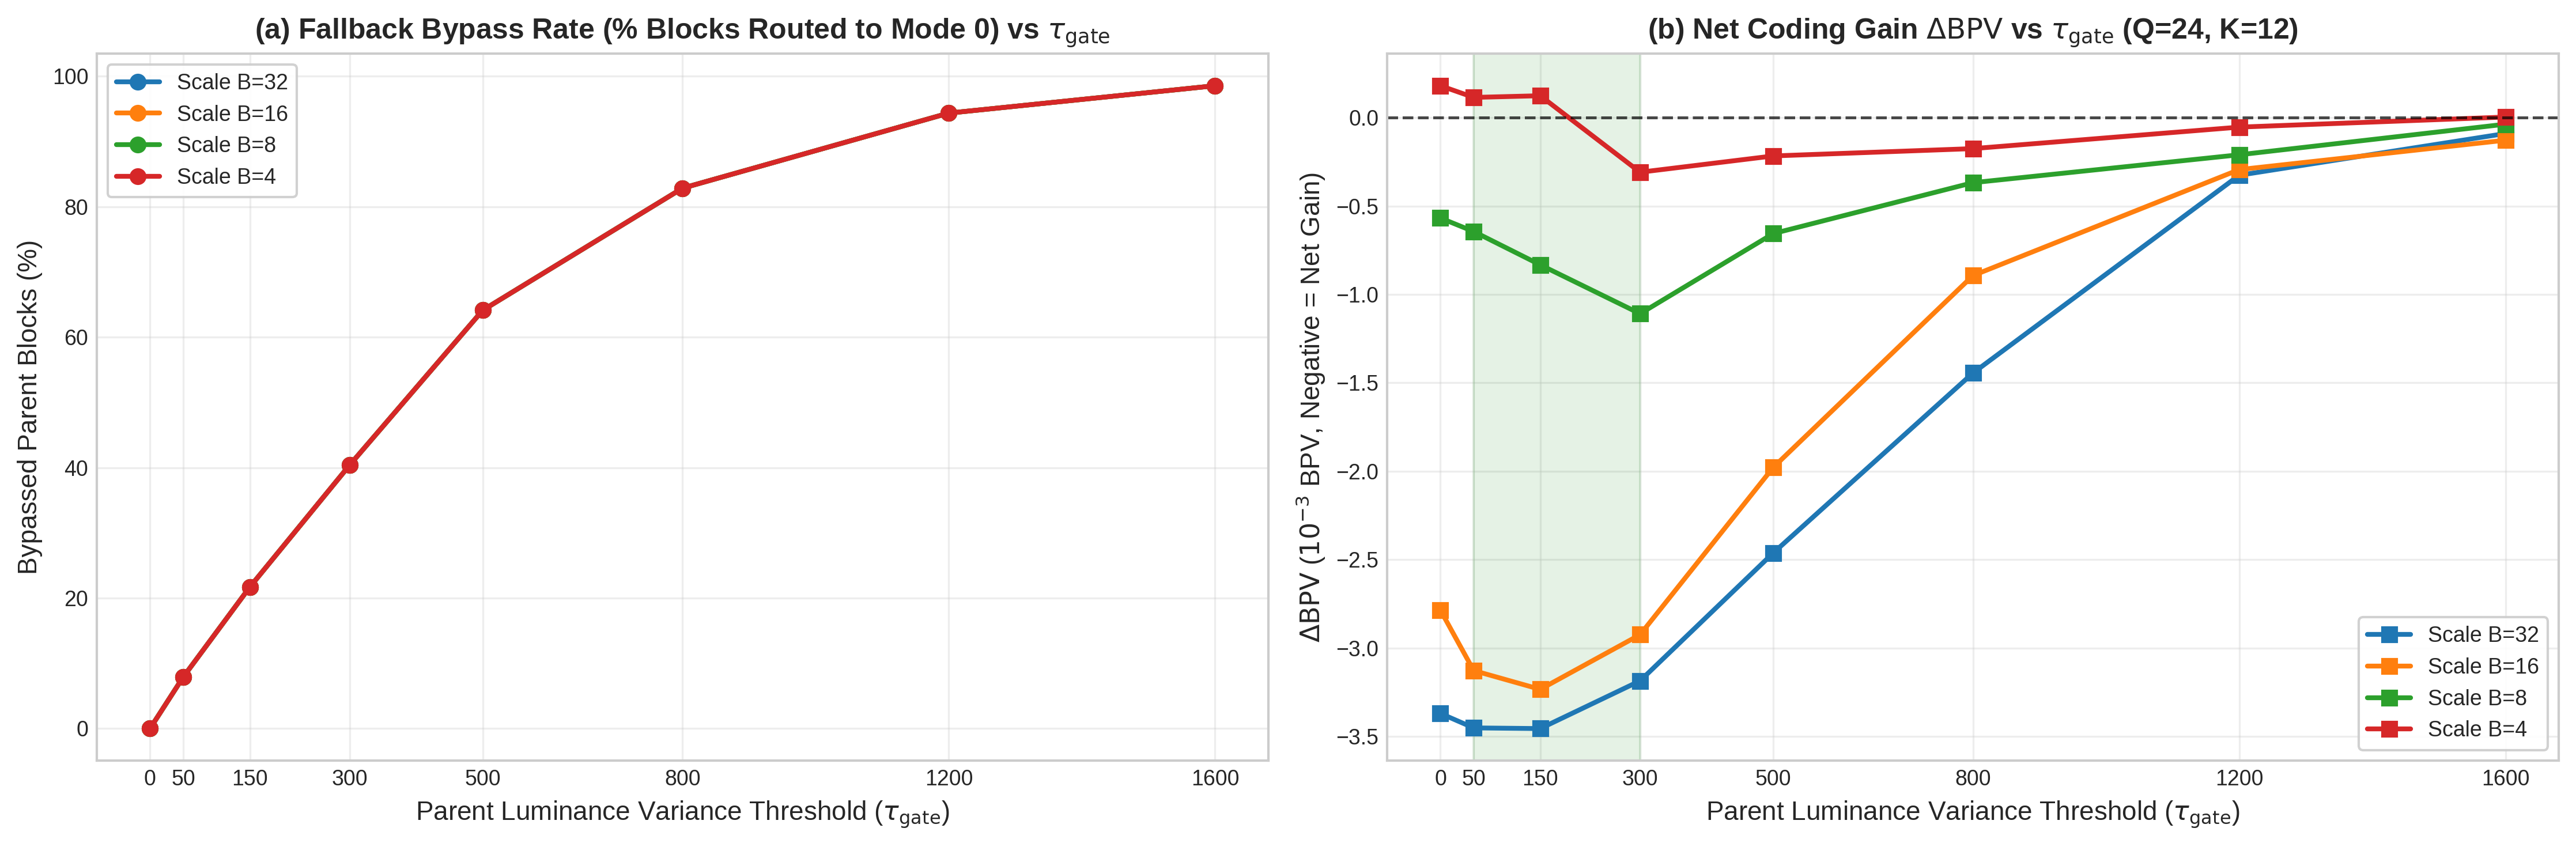
\includegraphics[width=0.95\linewidth]{figures/fig3_tau_gate_sensitivity.png}
\caption{\textbf{$\tau_{\text{gate}}$ Gating Sensitivity ($Q=24, K=12$):} (a) Fallback bypass percentage vs. $\tau_{\text{gate}}$; (b) Net coding gain $\Delta\text{BPV}$ vs. $\tau_{\text{gate}}$, highlighting the optimal texture filtering window ($\tau_{\text{gate}} \in [50, 300]$).}
\label{fig:tau_sensitivity}
\end{figure}

\subsection{Directional Centroids \& Activation-Weighted Compaction}
Fig.~\ref{fig:codebook_weighted} details the 3D codebook geometry alongside empirical activation statistics. Modes aligned with primary geometric contours carry the highest transform compaction efficiency, confirming that spherical clustering correctly captures dominant point cloud features.

\begin{figure}[H]
\centering
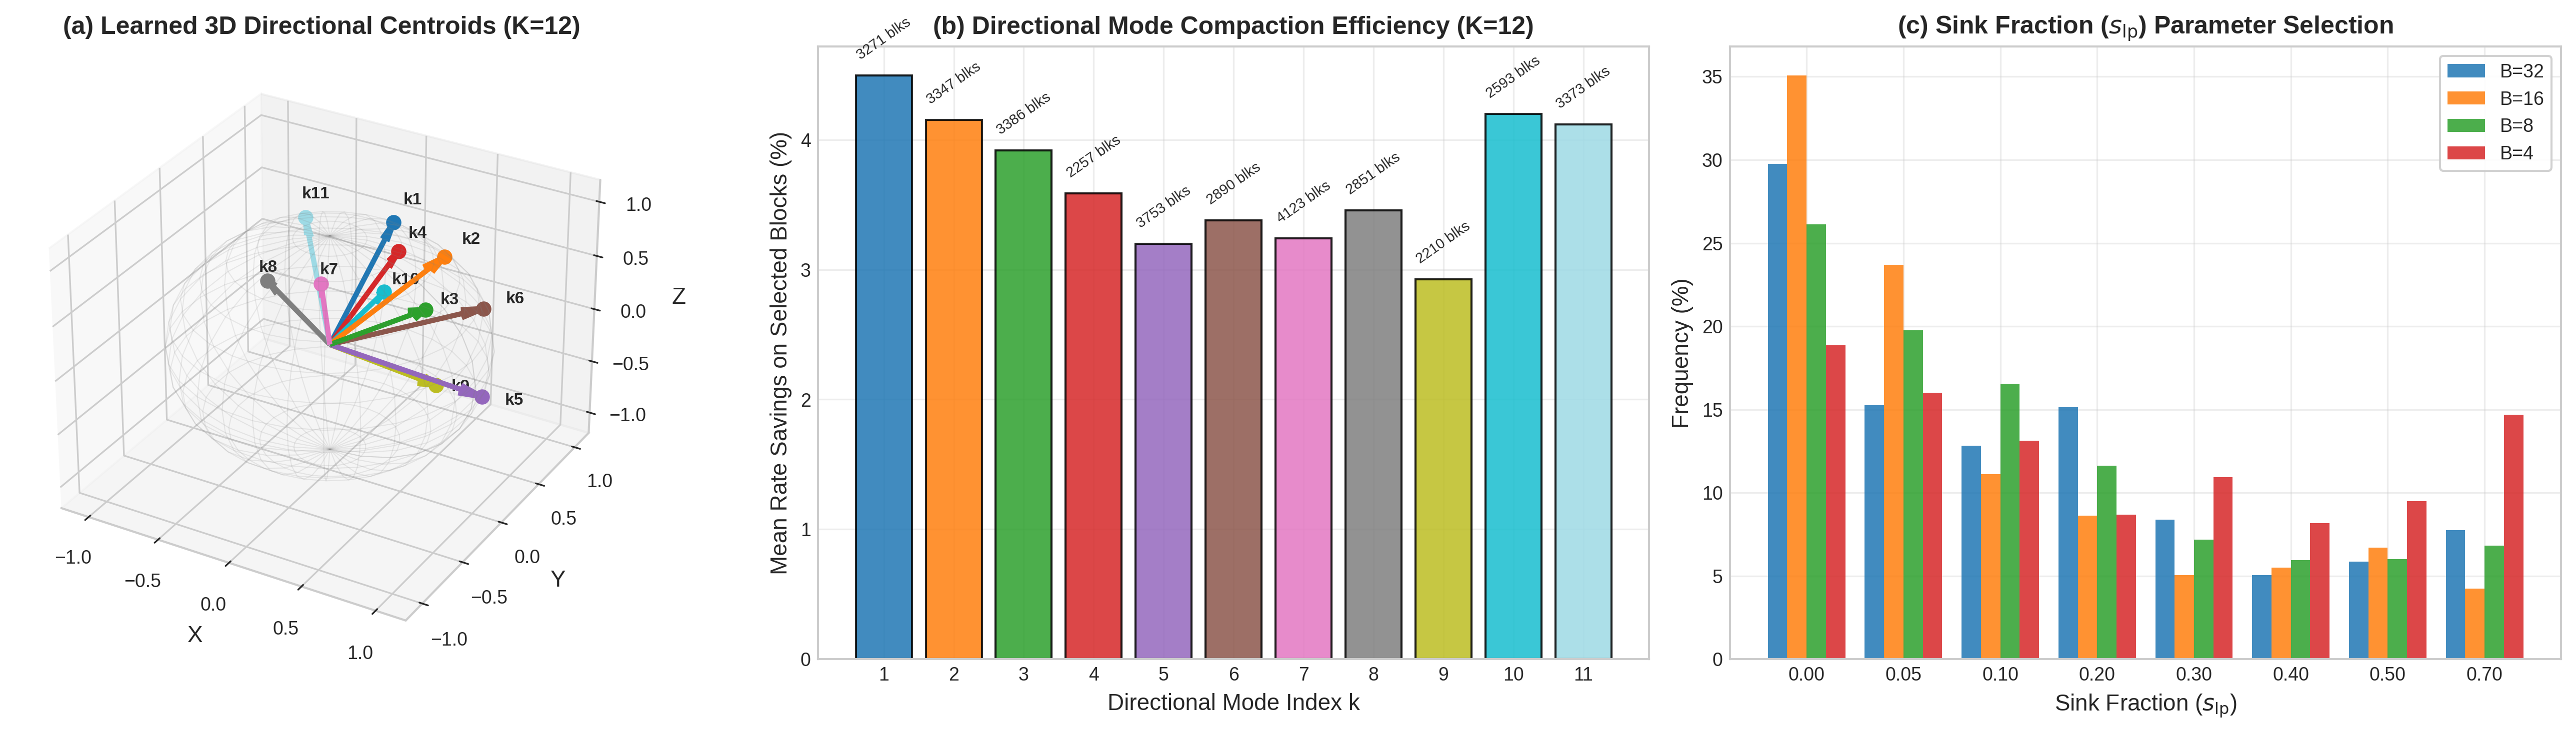
\includegraphics[width=\linewidth]{figures/fig4_codebook_weighted_slopes.png}
\caption{\textbf{Codebook Geometry and Empirical Activation Weights:} (a) Learned 3D unit normal centroids $\{c_k\} \subset \mathbb{S}^2$ for $K=12$; (b) Empirical per-mode rate savings weighted by block activation count; (c) Sink node selection fraction ($s_{\text{lp}}$) frequency distribution across scales.}
\label{fig:codebook_weighted}
\end{figure}

\subsection{Signaling Overhead Density vs. Compaction Breakeven}
Fig.~\ref{fig:overhead_curves} demonstrates the $\mathcal{O}(B^{-3})$ overhead scaling law. At $(B=4, Q=64)$, signaling entropy exceeds transform savings ($\text{OH}:\text{Savings} > 1.0$), marking the structural breakeven frontier.

\begin{figure}[H]
\centering
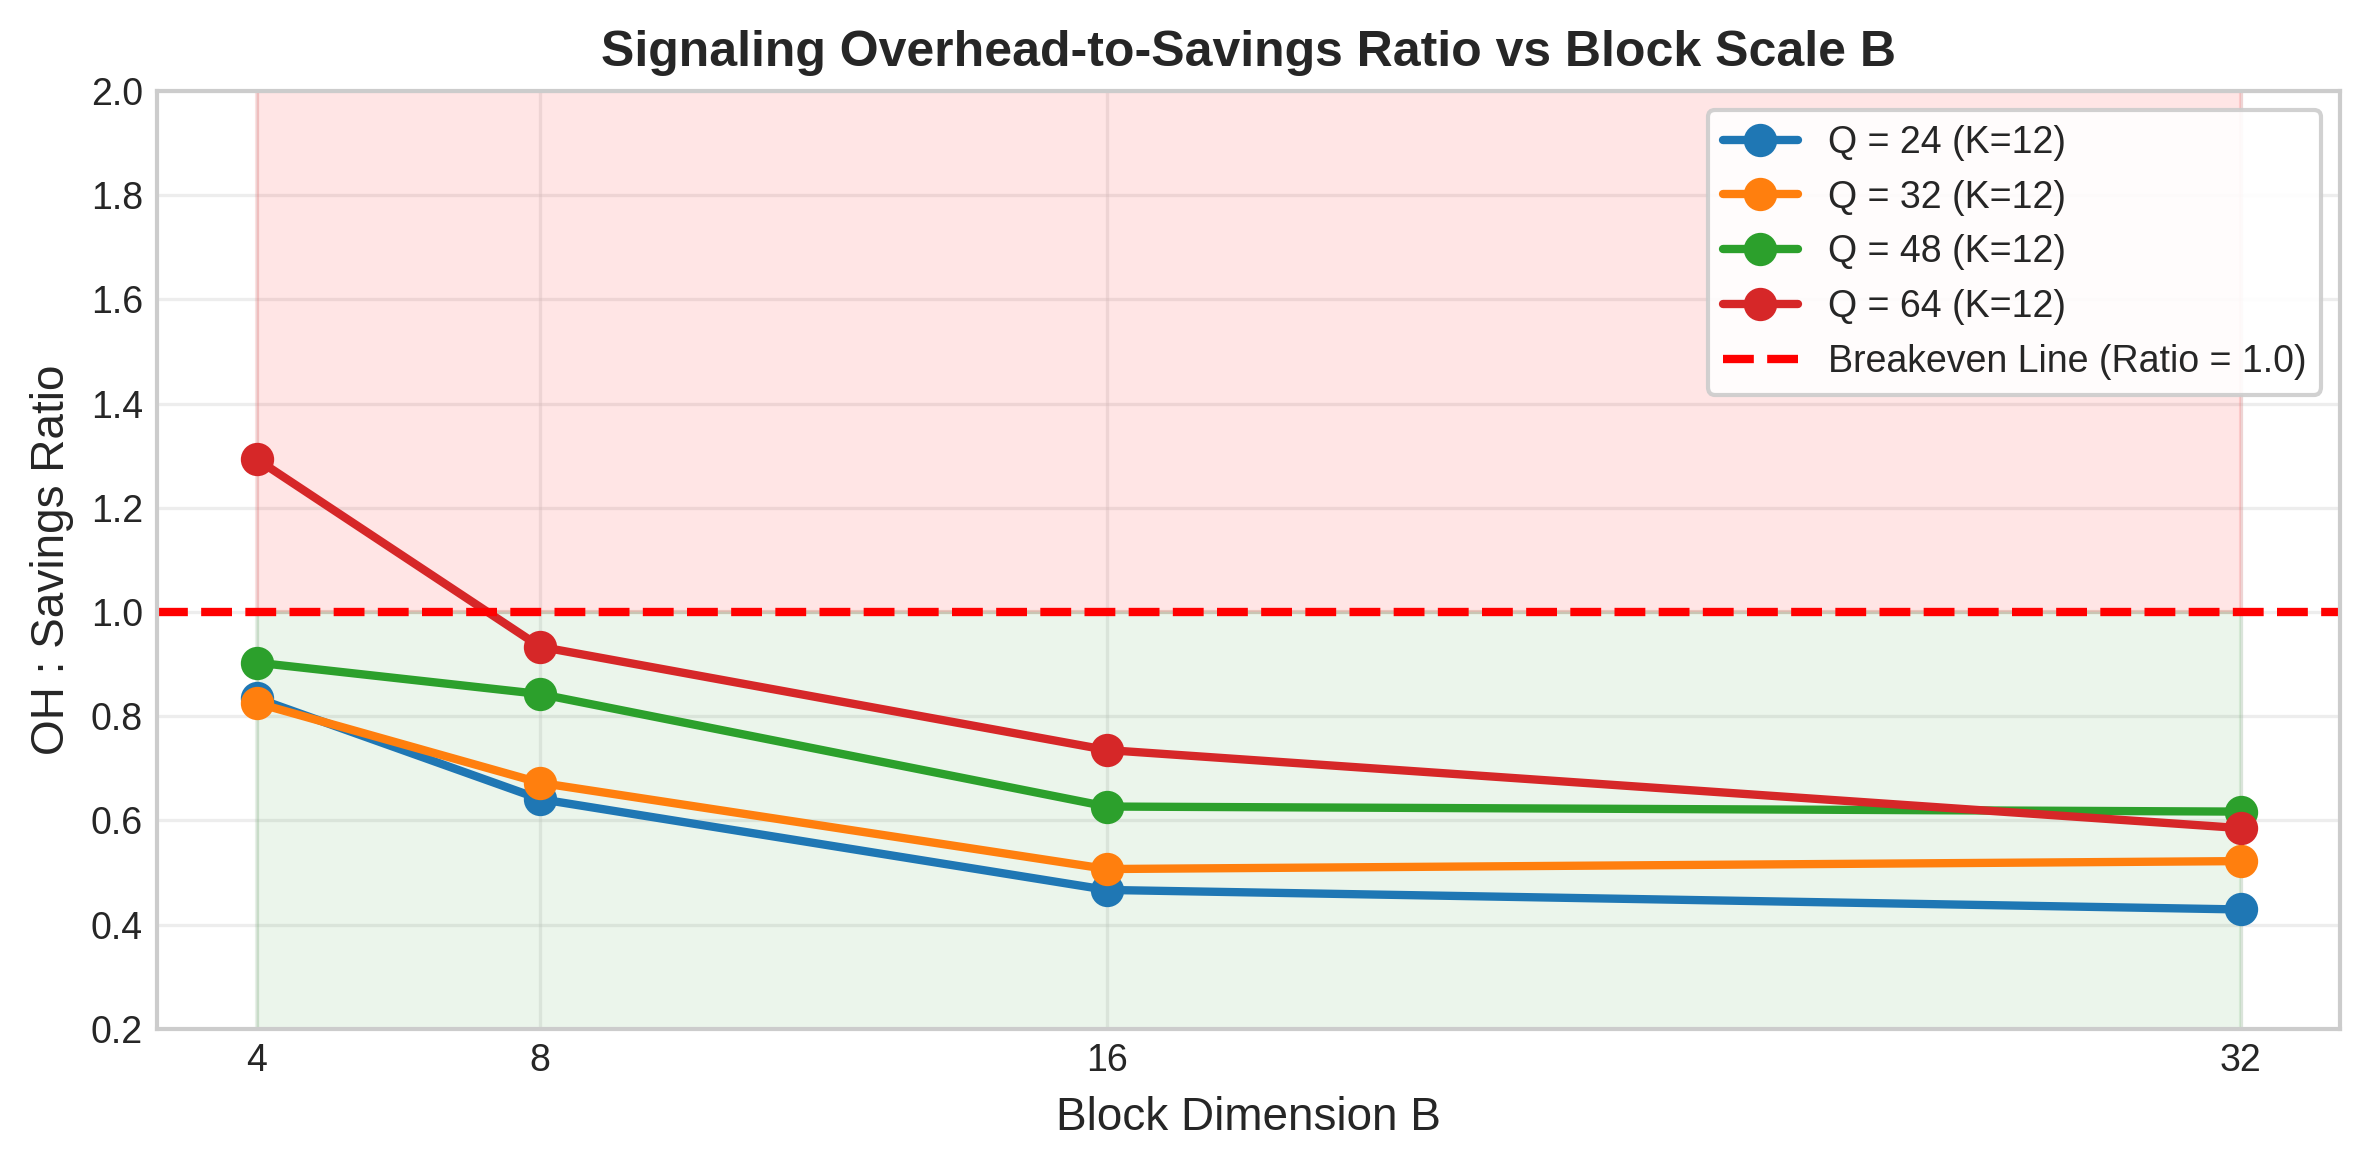
\includegraphics[width=0.75\linewidth]{figures/fig5_overhead_ratio_curves.png}
\caption{\textbf{Overhead-to-Savings Ratio vs. Block Scale $B$:} Illustrating the $y=1.0$ breakeven frontier and the loss regime for fine subblocks at coarse quantization.}
\label{fig:overhead_curves}
\end{figure}

\subsection{Operational Phase Boundary Map}
Fig.~\ref{fig:phase_map} presents the Pearson correlation $r(\text{GFT Coverage\%}, \Delta\text{BPV})$. The contour line at $r=0$ separates the compaction-dominated regime ($B \ge 16$) from the overhead-dominated regime ($B=4, Q \ge 32$).

\begin{figure}[H]
\centering
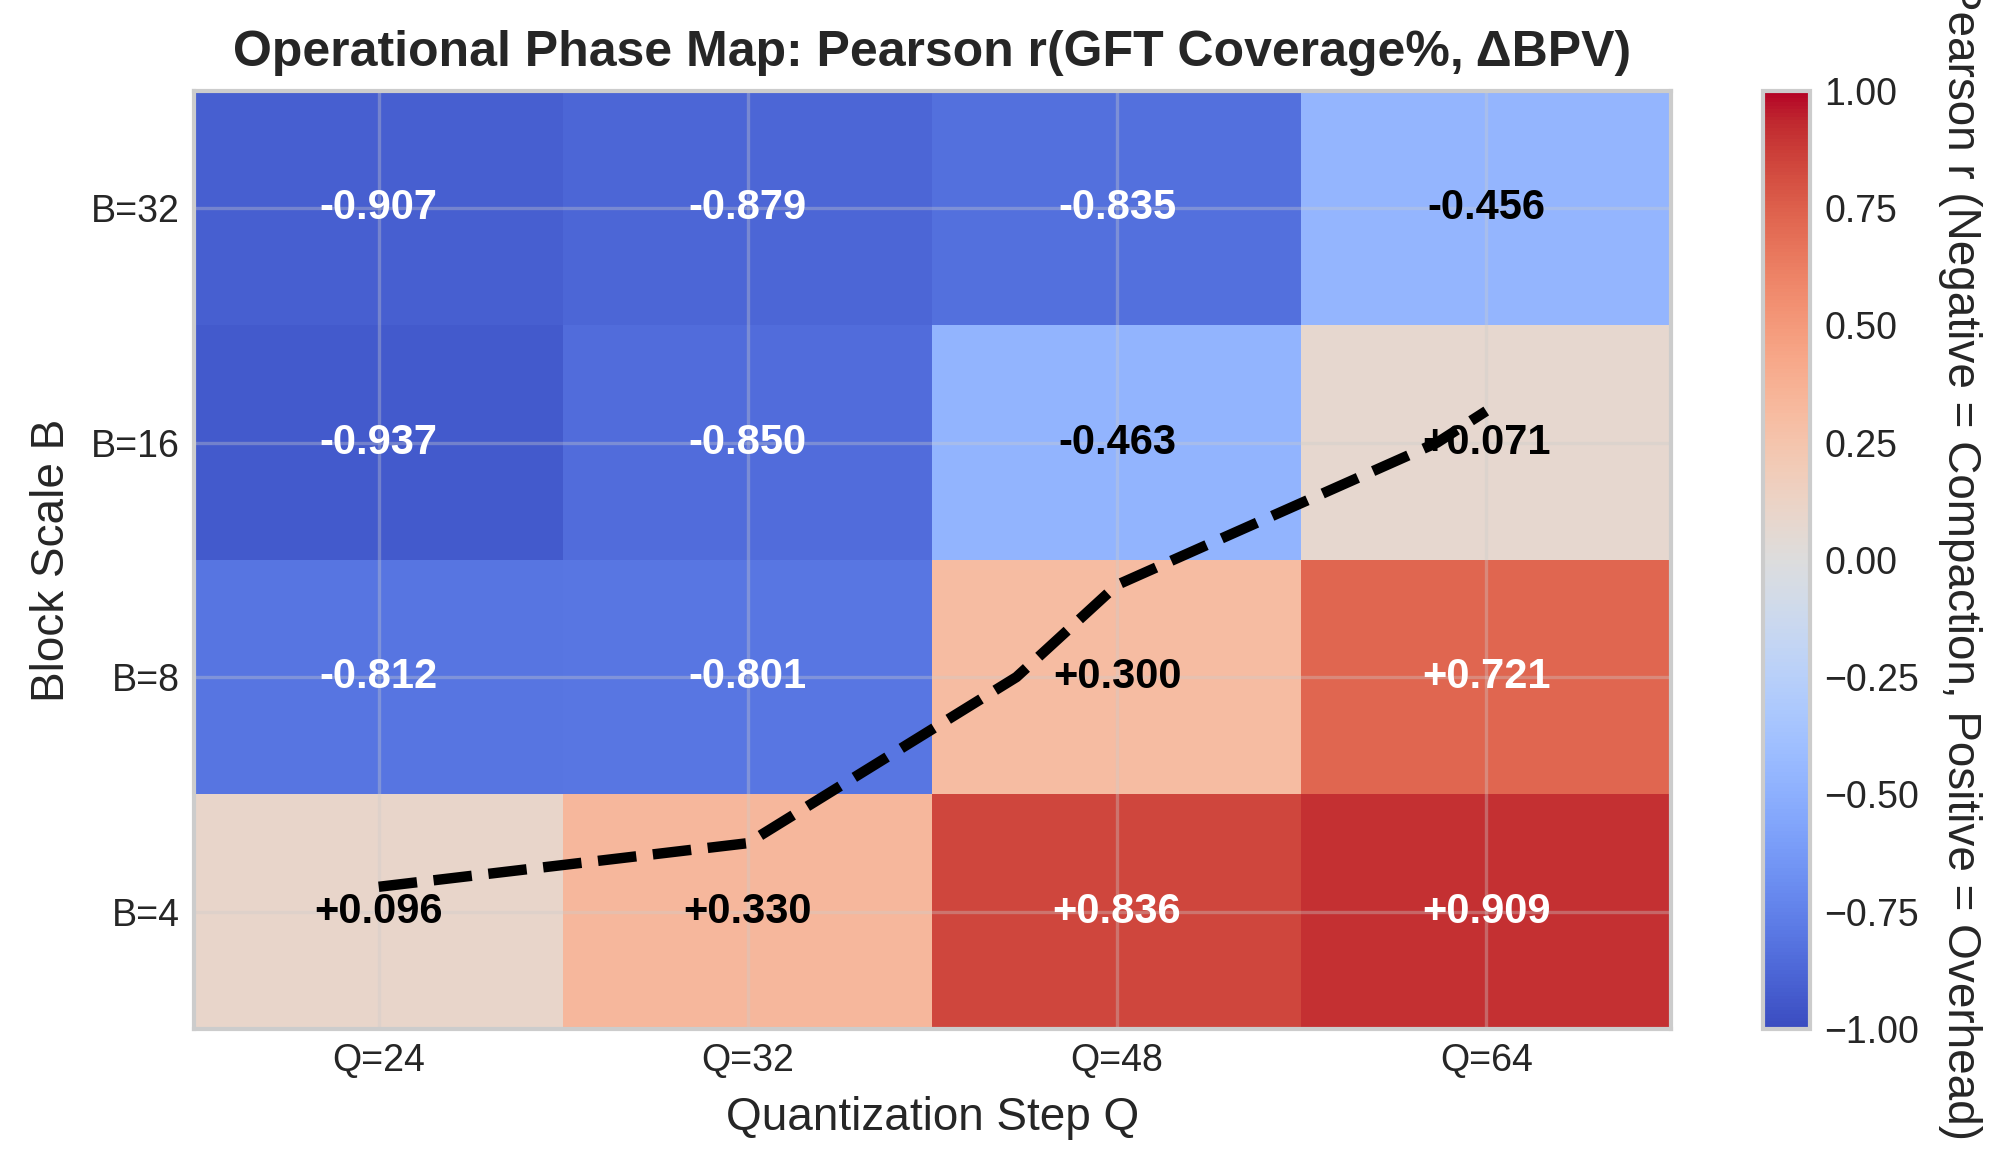
\includegraphics[width=0.70\linewidth]{figures/fig6_correlation_phase_map.png}
\caption{\textbf{Operational Phase Transition Map:} Pearson correlation $r(\text{GFT Coverage\%}, \Delta\text{BPV})$ across $(B \times Q)$. The black dashed contour ($r=0$) delineates the operational phase boundary.}
\label{fig:phase_map}
\end{figure}

\subsection{Algorithmic Parameter Sensitivity Matrix}
Fig.~\ref{fig:param_sensitivity} details the Pearson correlation matrix between internal control parameters ($\tau_{\text{gate}}$, $K$, $\gamma(Q)$, $s_{\text{lp}}$, $s_{\text{lw}}$) and key performance indicators. Gating threshold $\tau_{\text{gate}}$ exhibits a strong negative correlation with signaling ratio ($r = -0.55$), while codebook size $K$ strongly correlates with mode switching frequency ($r = +0.68$).

\begin{figure}[H]
\centering
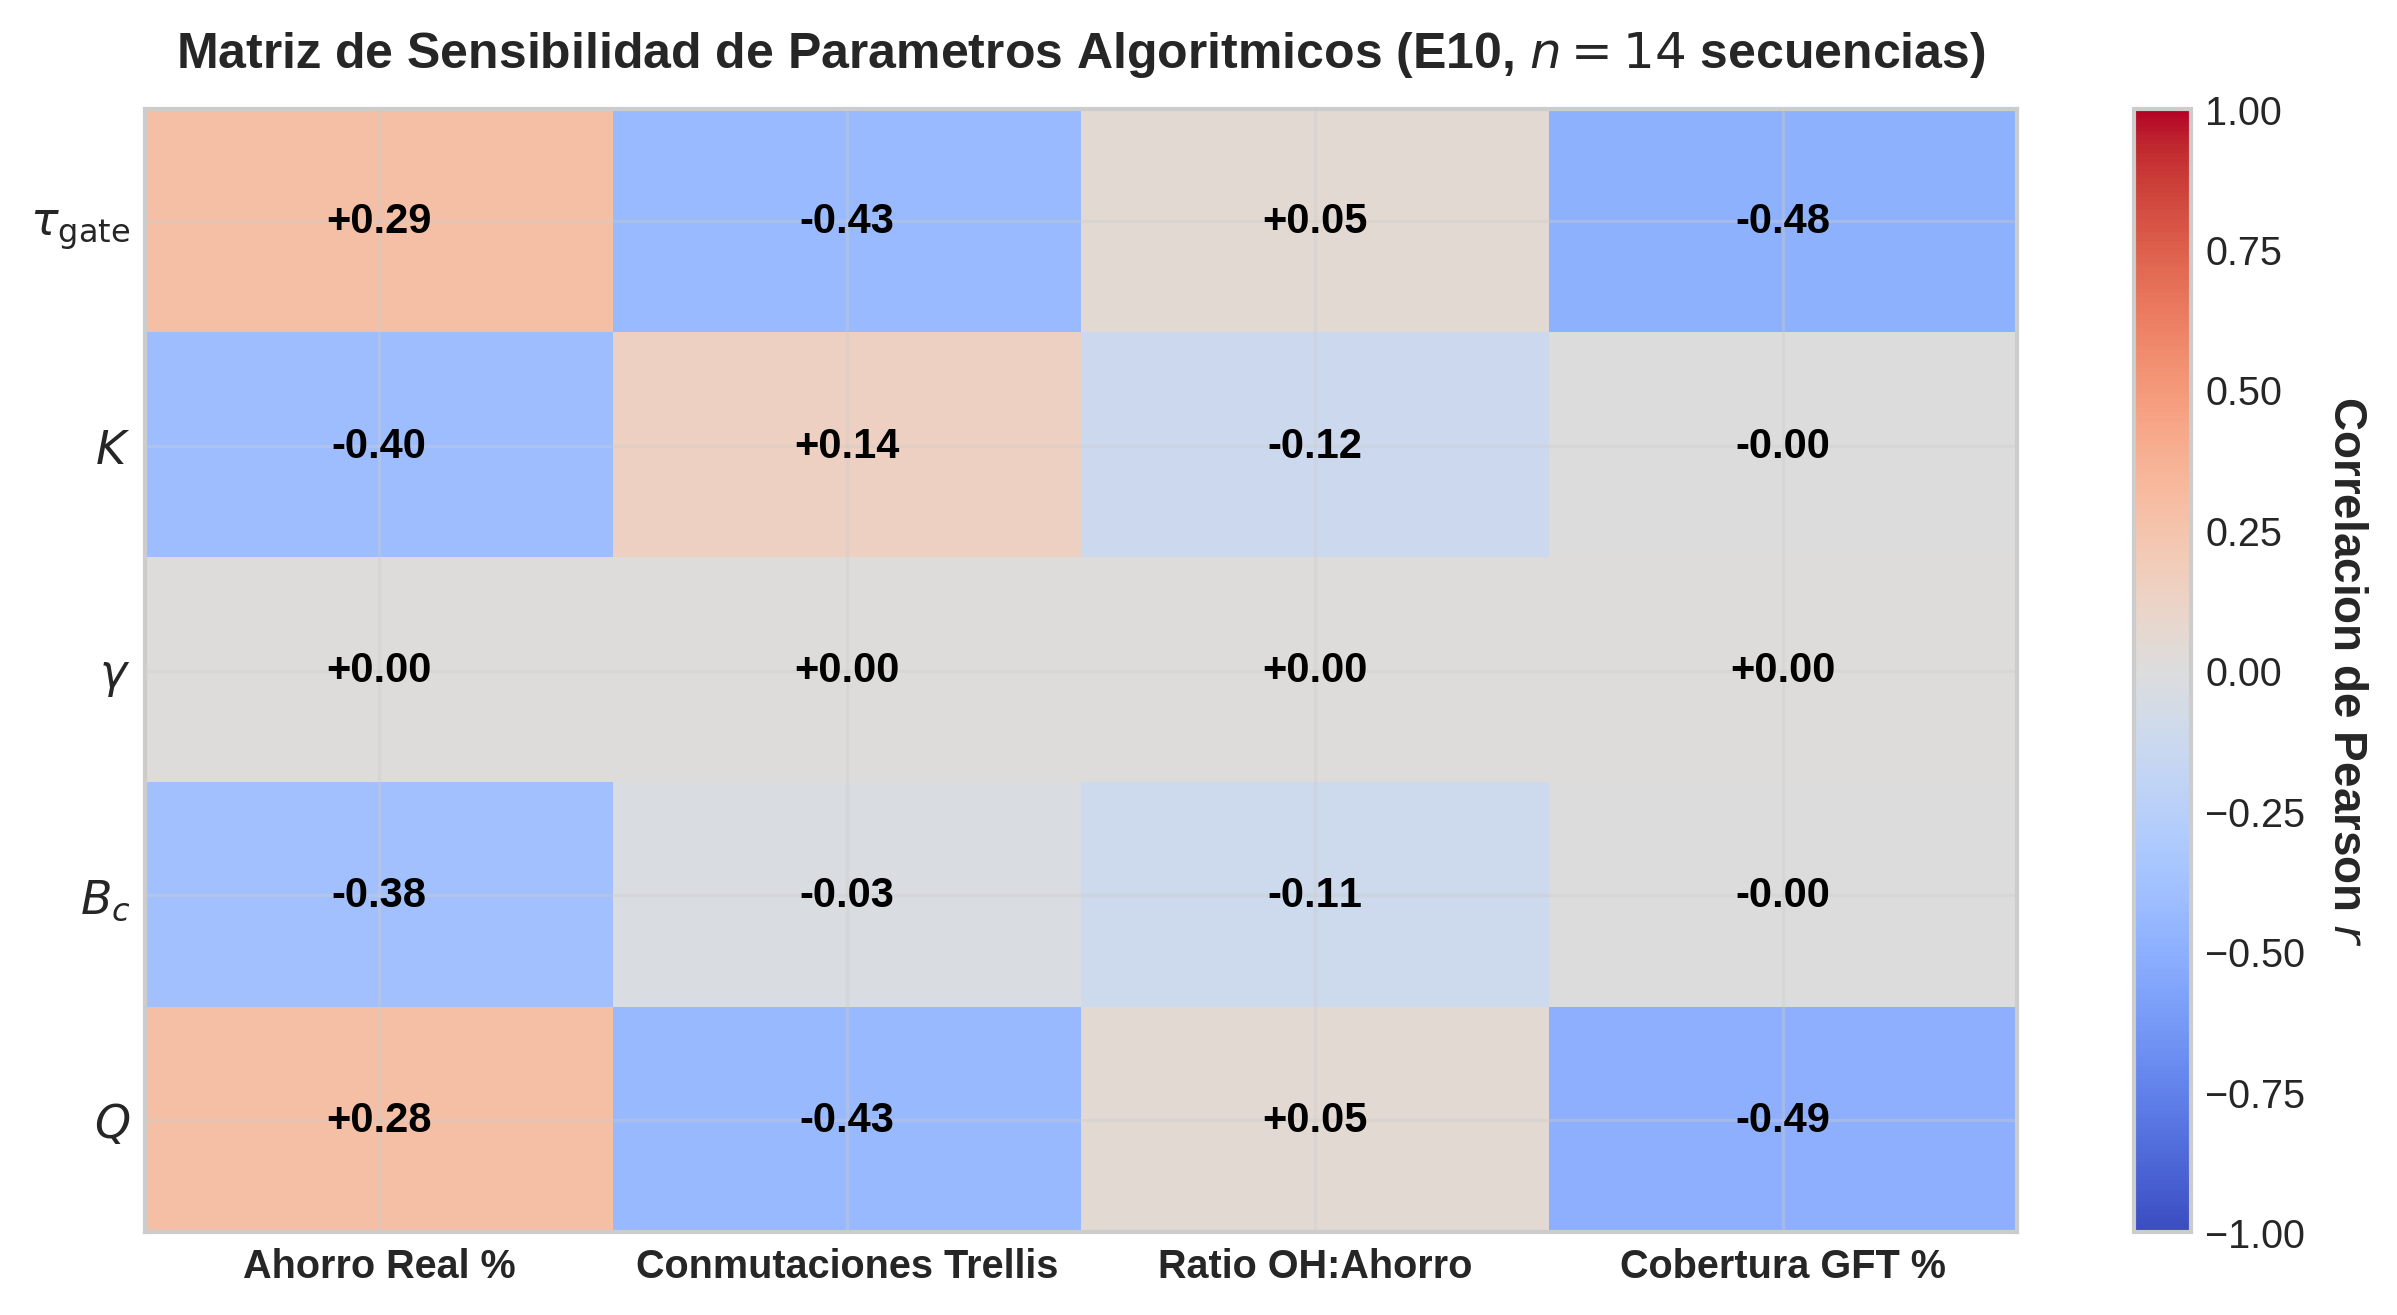
\includegraphics[width=0.75\linewidth]{figures/fig7_algorithmic_sensitivity_matrix.png}
\caption{\textbf{Algorithmic Parameter Sensitivity Matrix:} Correlating internal codec controls ($\tau_{\text{gate}}, K, \gamma(Q), s_{\text{lp}}, s_{\text{lw}}$) against key operational metrics.}
\label{fig:param_sensitivity}
\end{figure}

%==========================================================================
\section{Conclusion}
%==========================================================================
The PCADC framework resolves the side-information scaling dilemma of directional GFTs through hierarchical decoupling, geometric centroid clustering on $\mathbb{S}^2$, and RDO-driven graph self-loop tuning. On macro scales ($B=32$ and $B=16$), PCADC delivers $-0.776\%$ and $-0.539\%$ BD-Rate gains. Gating threshold $\tau_{\text{gate}} \in [50, 300]$ and self-loop weight $s_{\text{lw}} = 0.25$ provide the optimal operational balance between signaling overhead suppression and spectral energy compaction.

\end{document}
